\documentclass[pdflatex,sn-mathphys-num]{sn-jnl}

\usepackage{graphicx}
\usepackage{multirow}
\usepackage{amsmath,amssymb,amsfonts}
\usepackage{amsthm}
\usepackage{mathrsfs}
\usepackage[title]{appendix}
\usepackage{xcolor}
\usepackage{textcomp}
\usepackage{manyfoot}
\usepackage{booktabs}
\usepackage{algorithm}
\usepackage{algorithmicx}
\usepackage{algpseudocode}
\usepackage{listings}
\usepackage{tabularx}
\usepackage{array}
\usepackage{hyperref}

\raggedbottom

\begin{document}

\title[CoalGameRec: When Leave-One-Out Marginals Suffice]{CoalGameRec: When Leave-One-Out Marginals Suffice for Shapley-Based Graph Recommendation Attribution}

\author*[1]{\fnm{Mouad} \sur{Louhichi}}\email{mouad\_louhichi@um5.ac.ma}
\author[1]{\fnm{Redwane} \sur{Nesmaoui}}
\author[1]{\fnm{Mohamed} \sur{Lazaar}}

\affil*[1]{\orgdiv{National Higher School of Computer Science and Systems Analysis}, \orgname{ENSIAS, Mohammed V University in Rabat}, \orgaddress{\city{Rabat}, \country{Morocco}}}

\abstract{Shapley attribution is appealing for graph recommendation but costly, and its coalition averaging may be unnecessary for reranking. We study this boundary with CoalGameRec, a validation-guided interaction-attribution framework applied to a frozen LightGCN model. Historical interactions are players, coalition value is a validation-only pairwise log-sigmoid utility, and attribution is injected through item embeddings. We compare bounded Monte Carlo Shapley ($k=24$, $M=64$) with the grand-coalition leave-one-out (LOO) marginal on MovieLens-1M and Amazon-Book using temporal splits, full-catalog ranking, five seeds, and paired user bootstrap inference. LOO improves NDCG@20 over uniform reweighting by $8.1\%$ and $8.7\%$, respectively. Shapley also beats the non-game controls, but provides no practically meaningful NDCG@20 improvement over LOO: the pre-specified equivalence intervals lie within $\pm0.001$ and favor LOO on both datasets. LOO requires $13.0$--$15.7\times$ less attribution time. A confirmatory re-execution with validation-informed controls preserves the same ordering, while single-seed masked-forward tests provide limited evidence that both game-derived weights identify influential history. The contribution is therefore a scoped boundary result: under this LightGCN protocol, validation-guided marginal attribution is useful, whereas full Shapley averaging is not justified by ranking utility alone.}

\keywords{recommender systems, LightGCN, explainable AI, cooperative game theory, Shapley value, leave-one-out attribution, post-hoc reranking}

\maketitle

\section{Introduction}\label{sec:introduction}

Graph recommenders such as NGCF and LightGCN propagate preferences over user--item graphs and achieve strong top-$N$ ranking performance \cite{wang2019ngcf,he2020lightgcn,wu2022surveygnn}. Their predictions are nevertheless difficult to attribute to individual historical interactions, motivating work on explainable recommendation \cite{zhang2020explainable} and graph explanation.

Cooperative-game attribution defines players, coalition semantics, and a value function before allocating credit. This flexibility is also its main risk: a formally correct Shapley value may answer the wrong explanation question, inherit an additive similarity heuristic, or add substantial computation without improving ranking. Counterfactual recommenders, influence functions, and path-based graph reasoning provide important alternative views of interaction influence \cite{koh2017influence,ghazimatin2020prince,tran2021counterfactual,xian2019reinforcement}.

We therefore ask a narrow empirical question: under a frozen LightGCN protocol, does validation-guided interaction attribution improve reranking, and does Shapley averaging add value beyond the grand-coalition LOO marginal $v(N)-v(N\setminus\{j\})$? The protocol was frozen on July 15, 2026, before the final analyses. The study uses two datasets, five seeds, full-catalog temporal evaluation, and paired user-level inference. Claims are intentionally limited to this configuration.

\subsection{Contributions}\label{subsec:contributions}

The paper makes three scoped contributions.
\begin{enumerate}
    \item \textbf{Design guidance.} Five principles and a compact taxonomy make the player, coalition, value, solution, role, and intervention explicit, including the additive-leakage identity $\phi(v_{\mathrm{pref}})=\phi(v)+\lambda\,\mathrm{sim}$.
    \item \textbf{A boundary result.} Bounded Shapley beats matched non-game controls, but LOO is equivalent or better on NDCG@20 and requires $13.0$--$15.7\times$ less attribution time.
    \item \textbf{A reproducible test protocol.} Frozen splits and configurations, paired bootstrap inference, Holm correction, equivalence margins, and run artifacts support direct replication and extension.
\end{enumerate}

\section{Background and preliminaries}\label{sec:background}

\subsection{Graph-based top-N recommendation}\label{subsec:graph_rec}

Let $\mathcal{U}$ be the set of users and $\mathcal{I}$ the set of items. In implicit-feedback top-N recommendation, the observed training graph contains positive user-item interactions. A graph recommender learns user and item representations and produces a score $s(u,i)$ for each candidate item. Evaluation ranks all unseen eligible items for each user and measures whether the held-out item appears near the top.

This case study uses LightGCN as a graph recommender backbone \cite{he2020lightgcn}. Let $\mathbf{E}^{(0)}\in\mathbb{R}^{(|\mathcal{U}|+|\mathcal{I}|)\times d}$ be the layer-0 embeddings. With normalized adjacency $\tilde{\mathbf{A}}=\mathbf{D}^{-1/2}\mathbf{A}\mathbf{D}^{-1/2}$ of the training graph, LightGCN propagates
\begin{equation}
\mathbf{E}^{(l+1)} = \tilde{\mathbf{A}}\mathbf{E}^{(l)},\quad l=0,\dots,L-1,
\end{equation}
and reads out $\mathbf{e}_u = \frac{1}{L+1}\sum_{l=0}^{L} \mathbf{e}_u^{(l)}$, $\mathbf{e}_i$ likewise, scoring $s(u,i)=\langle \mathbf{e}_u,\mathbf{e}_i\rangle$. Training uses Bayesian Personalized Ranking \cite{rendle2009bpr}:
\begin{equation}
\mathcal{L}_{\text{BPR}} = -\sum_{(u,i,j)\in\mathcal{D}} \log\sigma(s(u,i)-s(u,j)) + \lambda_{\text{reg}}\|\Theta\|_2^2,
\end{equation}
where $i$ is a positive item, $j$ a sampled negative, $\sigma$ the sigmoid. In this paper LightGCN is the sole backbone (hypergraph variants are future work).

\subsection{Cooperative games and Shapley attribution}\label{subsec:shapley}

A cooperative game is defined by a player set $N$ and a characteristic function $v:2^N \rightarrow \mathbb{R}$ \cite{shapley1953value}. The SHAP framework \cite{lundberg2017shap} popularized Shapley for ML, and Data Shapley \cite{ghorbani2019datashapley} priced training points and efficient variants \cite{jia2019efficient}; ShaRP explains rankings \cite{pliatsika2025sharp}; we adapt the same axioms to interaction reranking. Beyond Shapley, robust alternatives for data valuation --- Banzhaf values \cite{wang2023banzhaf} and out-of-bag estimates \cite{kwon2023dataoob} --- and scalable model-behavior attribution \cite{park2023trak} show that simpler or non-Shapley value notions can be more stable under stochastic utility, consistent with our finding that the grand-coalition LOO marginal suffices for ranking. The Shapley value allocates the value of the grand coalition to players by averaging each player's marginal contribution over all coalition contexts. For player $p$,
\begin{equation}
\phi_p(v)=\sum_{S\subseteq N\setminus\{p\}} \frac{|S|!(|N|-|S|-1)!}{|N|!}\left[v(S\cup\{p\})-v(S)\right].
\end{equation}

In recommendation, $N$ may be a user's historical interactions. The value function may measure validation ranking utility when only a subset of those interactions is active. The Shapley value then assigns credit to historical interactions according to their expected contribution across contexts.

\subsection{Why Shapley may fail to add ranking value}\label{subsec:shapley_limits}

The Shapley value is not a guarantee of better recommendations. It is an allocation rule conditional on a chosen game. If the value function contains an additive similarity term, Shapley linearity decomposes that term into the same per-interaction similarity scores used by non-game baselines. If the value function uses hard top-20 NDCG with one validation item, many coalitions may receive zero utility, producing sparse marginal signals. If the intervention uses an external similarity kernel that is misaligned with the graph backbone, the attribution signal may be distorted before it affects ranking.

These issues motivated the case-study design used here. The primary game removes the additive preference term, uses a smooth validation-only pairwise utility, selects a stratified bounded player set, and applies attribution through the backbone-native item embedding space.

\section{A design framework for cooperative-game attribution}\label{sec:design_framework}

Shapley values are answers to specified games, not universal explanations. We use five design principles to make an attribution claim testable.

\subsection{Principle 1: the player must match the explanation question}\label{subsec:principle_player}

Players must match the explanation question: interactions support action-level explanations, graph edges support structural explanations, and providers support allocation questions \cite{yuan2021explainability}. Evidence for one player type does not automatically validate another.

\subsection{Principle 2: the value function must be smooth enough to attribute}\label{subsec:principle_value}

Hard top-$K$ utilities are flat for many coalitions. We therefore attribute a smooth validation-only pairwise utility and reserve HitRate and NDCG for final evaluation.
For user $u$, validation positive $i_u^+$, fixed validation negatives $\mathcal{N}_u^-$, and masked-graph scores $s_S$, the coalition value is
\begin{equation}\label{eq:pairwise}
v_u(S)=\frac{1}{|\mathcal{N}_u^-|}\sum_{i^-\in\mathcal{N}_u^-}\log\sigma\!\left(s_S(u,i_u^+)-s_S(u,i^-)\right).
\end{equation}
The test item is never used in this value, player selection, or tuning.

\subsection{Principle 3: additive terms should not be hidden inside Shapley claims}\label{subsec:principle_additive}

If the value function contains an additive term, Shapley linearity passes that term directly into the attribution. For example, if
\begin{equation}\label{eq:vpref}
v_{pref}(S)=v(S)+\lambda\sum_{j\in S}\mathrm{sim}(u,j),
\end{equation}
then
\begin{equation}\label{eq:phipref}
\phi_j(v_{pref})=\phi_j(v)+\lambda\mathrm{sim}(u,j).
\end{equation}
A Shapley method containing this term is partly a similarity method. The primary game therefore sets the additive coefficient to zero and evaluates similarity as a separate control.

\subsection{Principle 4: the intervention must be aligned with the model}\label{subsec:principle_intervention}

The intervention should be stated separately from the attribution rule. We use native LightGCN item embeddings in the primary protocol \cite{he2020lightgcn,wang2019ngcf}; the external-kernel ablation later shows that model alignment does not guarantee higher ranking accuracy.

\subsection{Attribution-guided reranking (exact intervention)}\label{subsec:reranking}
Let $a_j$ be the raw attribution for history item $j\in P_u$ (Shapley $\hat{\phi}_j$ or LOO $\phi^{\text{LOO}}_j$; both may be negative). Family weights are defined per family without pre-normalization:
\begin{equation}\label{eq:weights}
w_j = \begin{cases} a_j & \text{Shapley-MC / LOO (signed attributions)},\\ 1/|P_u| & \text{uniform},\\ \mathrm{softmax}_j\bigl(\cos(\mathbf{e}_j,\bar{\mathbf{e}}_u)/\tau\bigr) & \text{attention},\ \tau=0.10,\\ \max\bigl(0,\cos(\mathbf{e}_j,\bar{\mathbf{e}}_u)\bigr) & \text{additive-pref},\\ \log(1+\mathrm{deg}_j) & \text{heuristic-pop}, \end{cases}
\end{equation}
and the history representation is $\mathbf{r}_u = \sum_{j\in P_u} w_j \mathbf{e}_j$. With base scores $b_{ui}= \langle \mathbf{e}_u,\mathbf{e}_i\rangle$ and $\epsilon=10^{-12}$, final scores are
\begin{equation}\label{eq:rerank}
s'_{ui} = \mathrm{zscore}(b_{ui}) + \lambda_{\text{attr}}\cdot \mathrm{zscore}\bigl(\langle \mathbf{r}_u,\mathbf{e}_i\rangle\bigr),\quad \lambda_{\text{attr}}=0.10,
\end{equation}
The softmax is over $P_u$, and $\mathrm{deg}_j$ is the training-graph degree. For a candidate-score vector $x$, define
\[
\mathrm{zscore}(x)=\begin{cases}(x-\bar{x})/\mathrm{sd}(x),&\mathrm{sd}(x)>\epsilon,\\ \mathbf{0},&\mathrm{sd}(x)\le\epsilon.\end{cases}
\]
The implementation divides the attribution score by $d_u=\sum_j|w_j|+\epsilon>0$. Because this is a positive per-user scalar, it cannot reverse score signs and cancels under z-scoring whenever candidate variance is nonzero; the constant-score case maps to $\mathbf{0}$ in both forms. Shapley and LOO weights may be signed, but every family uses the same reranker. Candidates exclude training items, and the test item is never used for attribution or tuning.

\subsection{Principle 5: Shapley must be tested against marginal baselines}\label{subsec:principle_loo}

A credible Shapley claim must compare against the cheaper grand-coalition marginal $v(N)-v(N\setminus\{j\})$. If LOO matches Shapley, the useful signal comes from validation guidance rather than coalition-context averaging.

\subsection{Taxonomy, hypothesis, and scope}\label{sec:taxonomy}\label{sec:detailed_taxonomy}\label{sec:review_method}
We describe a method by six linked fields: player, coalition semantics, value, solution concept, attribution role, and graph structure. The evaluated slice uses interaction players, frozen edge masking, pairwise validation utility, Shapley or LOO allocation, reranking, and a bipartite LightGCN graph. The primary hypothesis is deliberately discriminative: both game-derived signals should beat matched non-game reweighting, while LOO should match or beat Shapley on ranking and cost. This single slice does not validate the taxonomy as a general theory.

\section{Related work and positioning}\label{sec:related_work}

Feature SHAP and Data Shapley allocate model output or data value to features and training points \cite{lundberg2017shap,ghorbani2019datashapley}. Influence functions offer a cheaper gradient-based route to training-point attribution \cite{koh2017influence}, while FastSHAP amortizes Shapley estimation with a learned explainer \cite{jethani2022fastshap}. These methods motivate alternatives but do not directly answer which historical interaction supports a recommendation.

Graph explainers identify nodes, edges, or subgraphs \cite{ying2019gnnexplainer,yuan2021explainability,duval2023graphsvx,zhang2022gstarx}. Recommendation-specific work instead includes knowledge-graph reasoning \cite{xian2019reinforcement}, provider-side counterfactual explanations \cite{ghazimatin2020prince}, and influence-based counterfactuals for neural recommenders \cite{tran2021counterfactual}. Their objectives differ from our post-hoc reranking intervention, so they are relevant external baselines for future validation rather than interchangeable evidence.

Recent work also cautions that perturbation fidelity can be misleading under graph distribution shift \cite{zheng2024robust,fang2023evaluating}. Accordingly, we separate ranking utility from explanation faithfulness and limit the empirical claim to the interaction-player LightGCN configuration shown in Fig.~\ref{fig:architecture}.


\begin{figure}[t]
\centering
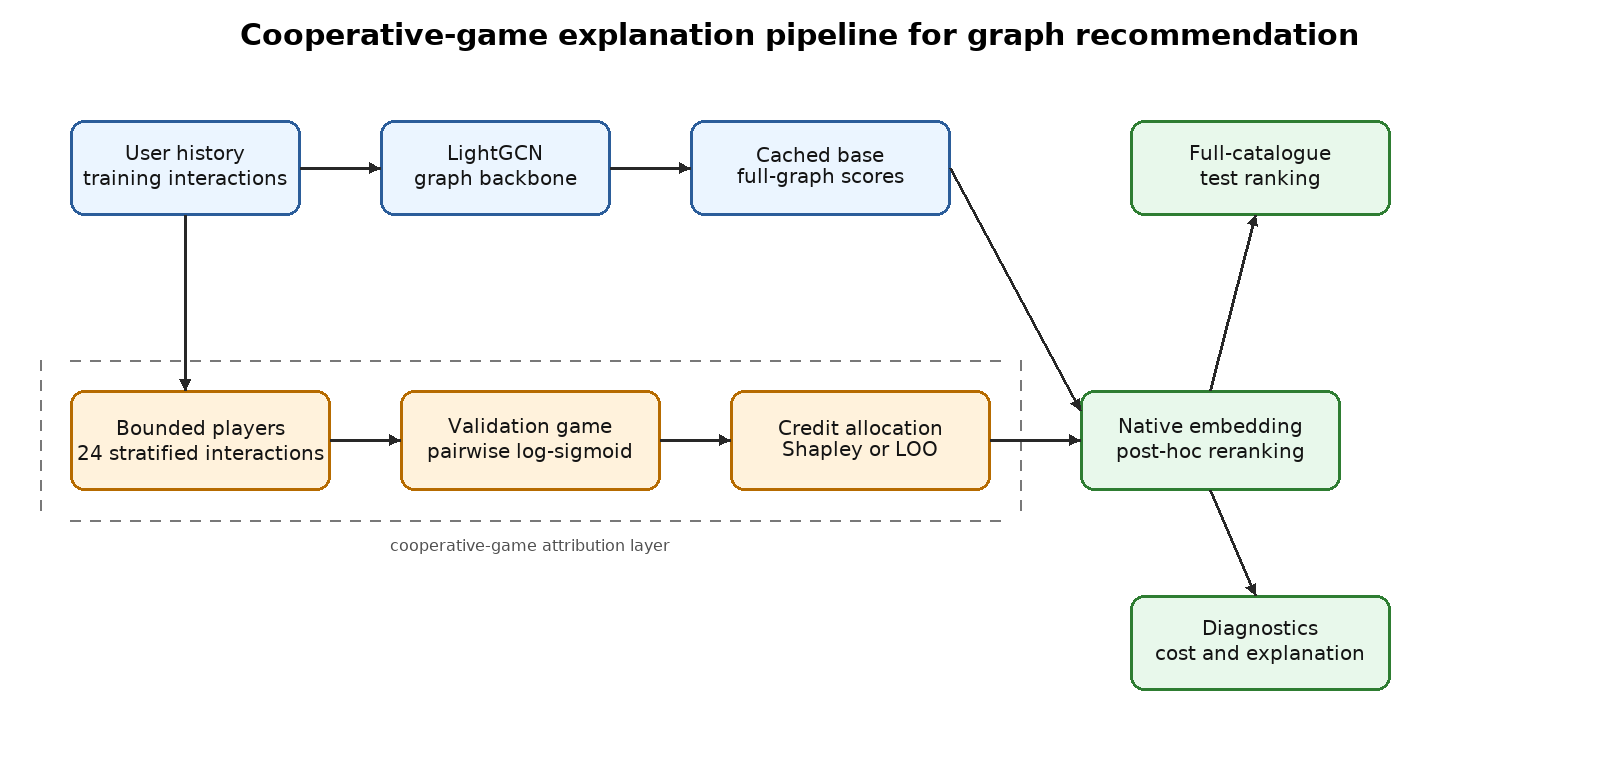
\includegraphics[width=\textwidth]{assets/figures/architecture.png}
\caption{CoalGameRec pipeline. A frozen LightGCN supplies base scores; a validation-only game attributes bounded historical interactions; Shapley or LOO weights then drive native-embedding reranking and separate cost/faithfulness diagnostics.}
\label{fig:architecture}
\end{figure}

\section{Method and complexity}\label{sec:algorithms}

Algorithms~\ref{alg:selection}--\ref{alg:rerank} formalise the pipeline in Fig.~\ref{fig:architecture} and match the released implementation. Algorithm~\ref{alg:shapley} seeds its permutation RNG with the run seed and returns an efficiency residual; Algorithm~\ref{alg:rerank} uses the stable z-score of \S\ref{subsec:reranking}. Similarity computations use train-only item vectors; the reranking intervention uses the native LightGCN embeddings. Hyperparameters are in Table~\ref{tab:hyper} (backbone) and Supplementary Table S3 (attribution/reranking).

\begin{algorithm}[t]
\caption{Stratified Bounded Player Selection}\label{alg:selection}
\begin{algorithmic}[1]
\Require User $u$, training history $H_u$, train-only item vectors $\{e_i\}$, val positive $i_u^+$, bound $k=24$
\Ensure Player set $P_u$, $|P_u|=\min(k,|H_u|)$ in deterministic order
\State Compute $\text{sim}_{\text{prof}}(j)=\cos(e_j,\bar e_u)$ where $\bar e_u=\frac{1}{|H_u|}\sum_{j\in H_u}e_j$
\State Compute $\text{sim}_{\text{val}}(j)=\cos(e_j,e_{i_u^+})$
\State Let $q=\lfloor k/3\rfloor$ and $r=k-3q$. Select $q$ profile-similar items for $P_1$, then $q$ validation-similar remaining items for $P_2$, then $q+r$ remaining items for $P_3$ by farthest-point sampling with cosine distance $1-\text{SafeCosine}$; ties use item id
\State $P_u\gets P_1\cup P_2\cup P_3$; if $|P_u|<\min(k,|H_u|)$, fill the remainder from $H_u\setminus P_u$ by $\text{sim}_{\text{prof}}$ order; sort by item id
\State Cosines use $\text{SafeCosine}(a,b)=a^\top b/(\|a\|\|b\|+\epsilon)$ (zero for a zero-norm vector); when $|H_u|<k$, missing slots are filled deterministically from the remaining profile-similarity order. Complexity with maintained minimum distances: $\mathcal{O}(k|H_u|d)$
\State \Return $P_u$
\end{algorithmic}
\end{algorithm}

\begin{algorithm}[t]
\caption{Validation-Only Coalition Value $v_u(S)$}\label{alg:value}
\begin{algorithmic}[1]
\Require User $u$, coalition $S\subseteq P_u$, val positive $i_u^+$, fixed val negatives $\mathcal{N}_u^-$ ($|\mathcal{N}_u^-|=100$), backbone $f_\theta$, train graph $G$
\Ensure Scalar $v_u(S)$ (Eq.~\ref{eq:pairwise})
\State $G_S\gets \text{MaskEdges}(G,\text{keep}=(H_u\setminus P_u)\cup S\text{ plus all training edges not incident to }u)$ \Comment{recompute degrees and $\tilde{A}_S$}
\State $\{e_x^S:x\in\mathcal{U}\cup\mathcal{I}\}\gets \text{LightGCNPropagate}(f_\theta,G_S)$; $s_S(u,i)=\langle e_u^S,e_i^S\rangle$
\State If $u$ has degree zero, its normalized-adjacency row is zero and the LightGCN readout retains its frozen layer-0 embedding
\State \Return $\frac{1}{|\mathcal{N}_u^-|}\sum_{i^-\in\mathcal{N}_u^-}\log\sigma(s_S(u,i_u^+)-s_S(u,i^-))$
\end{algorithmic}
\end{algorithm}

\begin{algorithm}[t]
\caption{Antithetic MC Shapley and LOO Marginal}\label{alg:shapley}
\begin{algorithmic}[1]
\Require $P_u$, value $v_u(\cdot)$, permutations $M=64$ (even), antithetic pairing, RNG seeded with the run seed
\Ensure $\hat\phi\in\mathbb{R}^{|P_u|}$, $\phi^{\text{LOO}}$
\State $\hat\phi\gets \mathbf{0}$; $v_\emptyset\gets v_u(\emptyset)$; $v_N\gets v_u(P_u)$
\For{$m=1$ to $M/2$}
  \State Sample $\pi\sim\text{Uniform}(S_{|P_u|})$; $\pi'\gets\text{Reverse}(\pi)$ \Comment{antithetic pair}
  \For{each permutation $\rho$ in the pair $(\pi,\pi')$}
    \State $S\gets\emptyset$; $prev\gets v_\emptyset$
    \For{$j$ in the order induced by $\rho$}
      \State $S\gets S\cup\{j\}$; $cur\gets v_u(S)$; $\hat\phi_j\gets\hat\phi_j+(cur-prev)$; $prev\gets cur$
    \EndFor
  \EndFor
\EndFor
\State $\hat\phi\gets\hat\phi/M$
\State $\phi^{\text{LOO}}_j\gets v_N-v_u(P_u\setminus\{j\})\;\forall j\in P_u$
\State $R_{\text{eff}}\gets\bigl|\sum_j\hat\phi_j-(v_N-v_\emptyset)\bigr|$ \Comment{diagnostic only; no residual redistribution}
\State \Return $\hat\phi$, $\phi^{\text{LOO}}$, $R_{\text{eff}}$
\end{algorithmic}
\end{algorithm}

\paragraph{Complexity.} Rebuilding degrees and normalized adjacency is $\mathcal{O}(|E_S|)$, and propagation plus utility evaluation costs $C_v=\mathcal{O}(L|E_S|d+|\mathcal{N}_u^-|d)$. Exact Shapley is $\mathcal{O}(2^kC_v)$, antithetic MC is $\mathcal{O}(MkC_v)$, and LOO is $\mathcal{O}((k+1)C_v)$. Reranking costs $\mathcal{O}(|\mathcal{C}_u|d)$ per user. Graph and embedding storage is $\mathcal{O}(|E|+|V|d)$, cached full-catalog scores are $\mathcal{O}(|\mathcal{U}||\mathcal{I}|)$, and stored bounded attributions are $\mathcal{O}(|\mathcal{U}|k)$. Measured attribution ratios are lower than the nominal $M$-fold gap because structures are cached and vectorized (Table~\ref{tab:cost}).


\begin{algorithm}[t]
\caption{Attribution-Guided Reranking}\label{alg:rerank}
\begin{algorithmic}[1]
\Require Family identifier $F$; base scores $b_{ui}$; candidate set $\mathcal{C}_u$; players $P_u$; embeddings $\mathbf{e}$; raw attributions $a_j$ (Shapley/LOO only); profile similarities and item degrees (heuristic families); $\lambda_{\text{attr}}$, $\tau$, $\epsilon$
\Ensure Reranked list
\State Compute family weights $w_j$ exactly as in Eq.~(\ref{eq:weights}) (raw signed $a_j$ for Shapley/LOO; no pre-normalization)
\State $\mathbf{r}_u \gets \sum_{j\in P_u} w_j \mathbf{e}_j$;\quad $d \gets \sum_{j\in P_u}|w_j|+\epsilon$ \Comment{numerically safe; cancels under z-scoring (\S\ref{subsec:reranking})}
\For{$i\in\mathcal{C}_u$}
\State $s'_{ui} \gets \mathrm{zscore}(b_{ui}) + \lambda_{\text{attr}}\cdot\mathrm{zscore}\bigl(\langle\mathbf{r}_u,\mathbf{e}_i\rangle/d\bigr)$
\EndFor
\State \Return $\mathcal{C}_u$ sorted by $s'_{ui}$, with deterministic item-id tie-breaking (including the all-equal case)
\end{algorithmic}
\end{algorithm}
\section{Experimental setup}\label{sec:protocol_details}\label{sec:case_study}

\subsection{Scope, data, and leakage control}\label{subsec:leakage}\label{subsec:case_scope}\label{subsec:data_splits}

The study evaluates one configuration only: interaction players, frozen LightGCN edge masking, validation pairwise utility, Shapley or LOO allocation, and post-hoc reranking. We use MovieLens-1M \cite{harper2015movielens} and a temporal Amazon-Book split derived from Amazon Reviews 2018 Books 5-core \cite{ni2019justifying}. Table~\ref{tab:datasets} reports the processed data; Amazon is substantially sparser.

\begin{table}[t]
\caption{Processed temporal datasets. Density and averages use training interactions only.}\label{tab:datasets}
\centering
\small
\begin{tabular}{lrrrrrr}
\toprule
Dataset & Users & Items & Train & Val. & Test & Density / train per user \\
\midrule
ML-1M & 6{,}015 & 3{,}114 & 562{,}183 & 6{,}015 & 6{,}015 & 3.001\% / 93.46 \\
Amazon-Book & 7{,}417 & 12{,}885 & 109{,}915 & 7{,}417 & 7{,}417 & 0.115\% / 14.82 \\
\bottomrule
\end{tabular}
\end{table}

Ratings of at least four stars are positives. After a stable temporal ordering and iterative training-period 5-core filter, the last positive is test, the second-last is validation, and earlier positives form the training graph. Training items are excluded from candidates; ranking uses the full remaining catalog. Similarity vectors, player selection, and model training use training data only. Coalition values use validation items only, and test items are reserved for final evaluation. For 24\% of ML-1M users and 89\% of Amazon users, the bounded $k=24$ game covers the full training history.

\subsection{Evaluation protocol}\label{subsec:evaluation_protocol}

For each evaluated user, all training items are excluded from the candidate list. The held-out test item remains in the candidate set. The model ranks the full eligible catalog, not a sampled negative pool. HitRate@K equals one if the held-out test item is in the top K and zero otherwise. NDCG@K is the reciprocal log discount of the held-out item's rank when it appears in the top K. Coverage@20 is the fraction of the global eligible item catalog appearing in at least one user's top-20 list. ILD@20 is computed from the train-only item similarity representation.

\subsection{Metrics}\label{subsec:metrics_formal}
For user $u$ with test item $i_u^{\text{test}}$ and candidate set $\mathcal{C}_u=\mathcal{I}\setminus H_u^{\text{train}}$, let $\text{rank}_u\in[1,|\mathcal{C}_u|]$ be the rank of $i_u^{\text{test}}$ under scores $s(u,\cdot)$. Then
$\text{HitRate}_u@K=\mathbf{1}[\text{rank}_u\le K]$,
$\text{NDCG}_u@K=\mathbf{1}[\text{rank}_u\le K]/\log_2(\text{rank}_u+1)$ (binary relevance, IDCG$=1$),
$\text{Coverage}@K=|\bigcup_u \text{Top}_K(u)|/|\mathcal{I}_{\text{eligible}}|$,
$\text{ILD}@K(u)=1-\frac{2}{K(K-1)}\sum_{a<b}\cos(e_a,e_b)$ averaged over users (train-only item vectors $e$). Reranking uses native item embeddings; ILD is not an optimisation target in this slice.

\subsection{Statistical estimand}\label{subsec:stat_estimand}

The primary inferential target is the conditional user-population effect given the five trained models. For seeds $s=1..5$ we resample users with replacement within each seed ($B=2000$ paired bootstrap replicates, seed 20260804), compute seed-specific mean differences $\Delta_s$, and average $\bar\Delta=\frac{1}{5}\sum_s\Delta_s$; 95\% CIs are percentile intervals over $B$ replicates. The primary family is defined explicitly: per dataset, $F=8$ contrasts, Shapley-MC vs.\ each of uniform, additive-pref, attention, and LOO on NDCG@20 and HitRate@20, Holm-corrected within the family. Coverage/ILD and the descriptive 5-seed means are exploratory and carry no paired contrasts. Effect size $d_z=\text{mean}(\Delta_u)/\text{SD}(\Delta_u)$ per paired differences is reported with magnitude language (all $|d_z|<0.08$ = negligible). This estimand does not claim uncertainty over all possible model initializations; seed variability is descriptive (mean$\pm$SD over 5 seeds). The bootstrap hierarchy resamples users within each seed and averages seed-specific means; the same users appear under all five trained models, so the procedure captures user-level variation conditional on the five models and treats the models as fixed. We report this as the declared estimand rather than claiming fully hierarchical cross-model calibration.

Bootstrap p-values are two-sided sign probabilities: with $\Delta^*_b$ the $b$-th replicate of the mean-of-seed-means statistic, $\hat{p}=2\min(\#\{\Delta^*_b\le0\}/B,\ \#\{\Delta^*_b\ge0\}/B)$, reported as ``$<1/B$'' when the count is zero ($B=2000$). Holm--Bonferroni step-down correction at $\alpha=0.05$ is applied within each pre-specified family ($F=8$ primary; $F=10$ LOO-as-treatment; $F=12$ C1); the families are declared a priori and corrected independently.

For equivalence we pre-specify a smallest effect size of practical interest (SESOI): $\delta=0.001$ for NDCG@20 and $\delta=0.002$ for HitRate@20, approximately one quarter of the LOO-vs-uniform improvement under this protocol; effects inside $(-\delta,\delta)$ are declared practically negligible. Following the TOST--CI equivalence, equivalence holds when the 90\% bootstrap percentile CI of the Shapley--LOO difference lies entirely inside $(-\delta,\delta)$. Results are reported in Table~\ref{tab:equivalence}.

\subsection{Backbone and comparators}\label{subsec:families}

The graph backbone is LightGCN with two propagation layers, trained with a Bayesian personalized ranking objective \cite{rendle2009bpr,he2020lightgcn}. We train for five seeds $\{42,43,44,45,46\}$. The attribution families are:
\begin{itemize}
    \item \textbf{uniform:} all historical interactions receive equal weight.
    \item \textbf{additive-pref:} weights are direct positive similarity to the user's training profile.
    \item \textbf{attention:} fixed attention-style softmax over profile similarity.
    \item \textbf{heuristic-pop:} popularity-weighted historical interactions.
    \item \textbf{loo-marginal:} leave-one-out marginal value $v(N)-v(N\setminus\{j\})$.
    \item \textbf{shapley-mc:} antithetic permutation Monte Carlo Shapley over a bounded stratified set of 24 historical interactions.
\end{itemize}

The Shapley game omits additive preference. Its coalition value is a smooth, validation-only pairwise log-sigmoid utility. The final reranker applies attribution through the native item embedding space.

\subsection{Hyperparameters (shared across families)}\label{subsec:hyper}
Table~\ref{tab:hyper} lists backbone and attribution hyperparameters (resolved from the frozen run configuration files). Reranking weight $\lambda_{\text{attr}}=0.10$ and temperature $\tau=0.10$ were fixed a priori and shared across families; the sensitivity sweep over $\lambda_{\text{attr}}\in\{0.00,0.05,0.10,0.20,0.40\}$ (Table~\ref{tab:ablation_lambda}) is reported for interpretation only and was never used to select family-specific $\lambda$.

\begin{table}[t]
\caption{Key hyperparameters (shared across families unless noted).}\label{tab:hyper}
\centering
\small
\resizebox{\textwidth}{!}{
\begin{tabular}{lll}
\toprule
Component & Parameter & Value \\
\midrule
LightGCN & layers / dim / lr / wd / epochs / batch / neg & 2 / 64 / 0.002 / 1e-5 / 15 / 4096 / 2 \\
Attribution & $k$ / $M$ / $|\mathcal{N}_u^-|$ / antithetic / value & 24 / 64 / 100 / true / pairwise log-sigmoid \\
Reranking & intervention / $\lambda_{\text{attr}}$ / $\tau$ & native item-embedding / 0.10 / 0.10 \\
Evaluation & $K$ / seeds / ranking & \{5,10,20\} / 42--46 / full-catalog \\
\bottomrule
\end{tabular}
}
\end{table}

\section{Results}\label{sec:results}

\begin{figure*}[t]
\centering
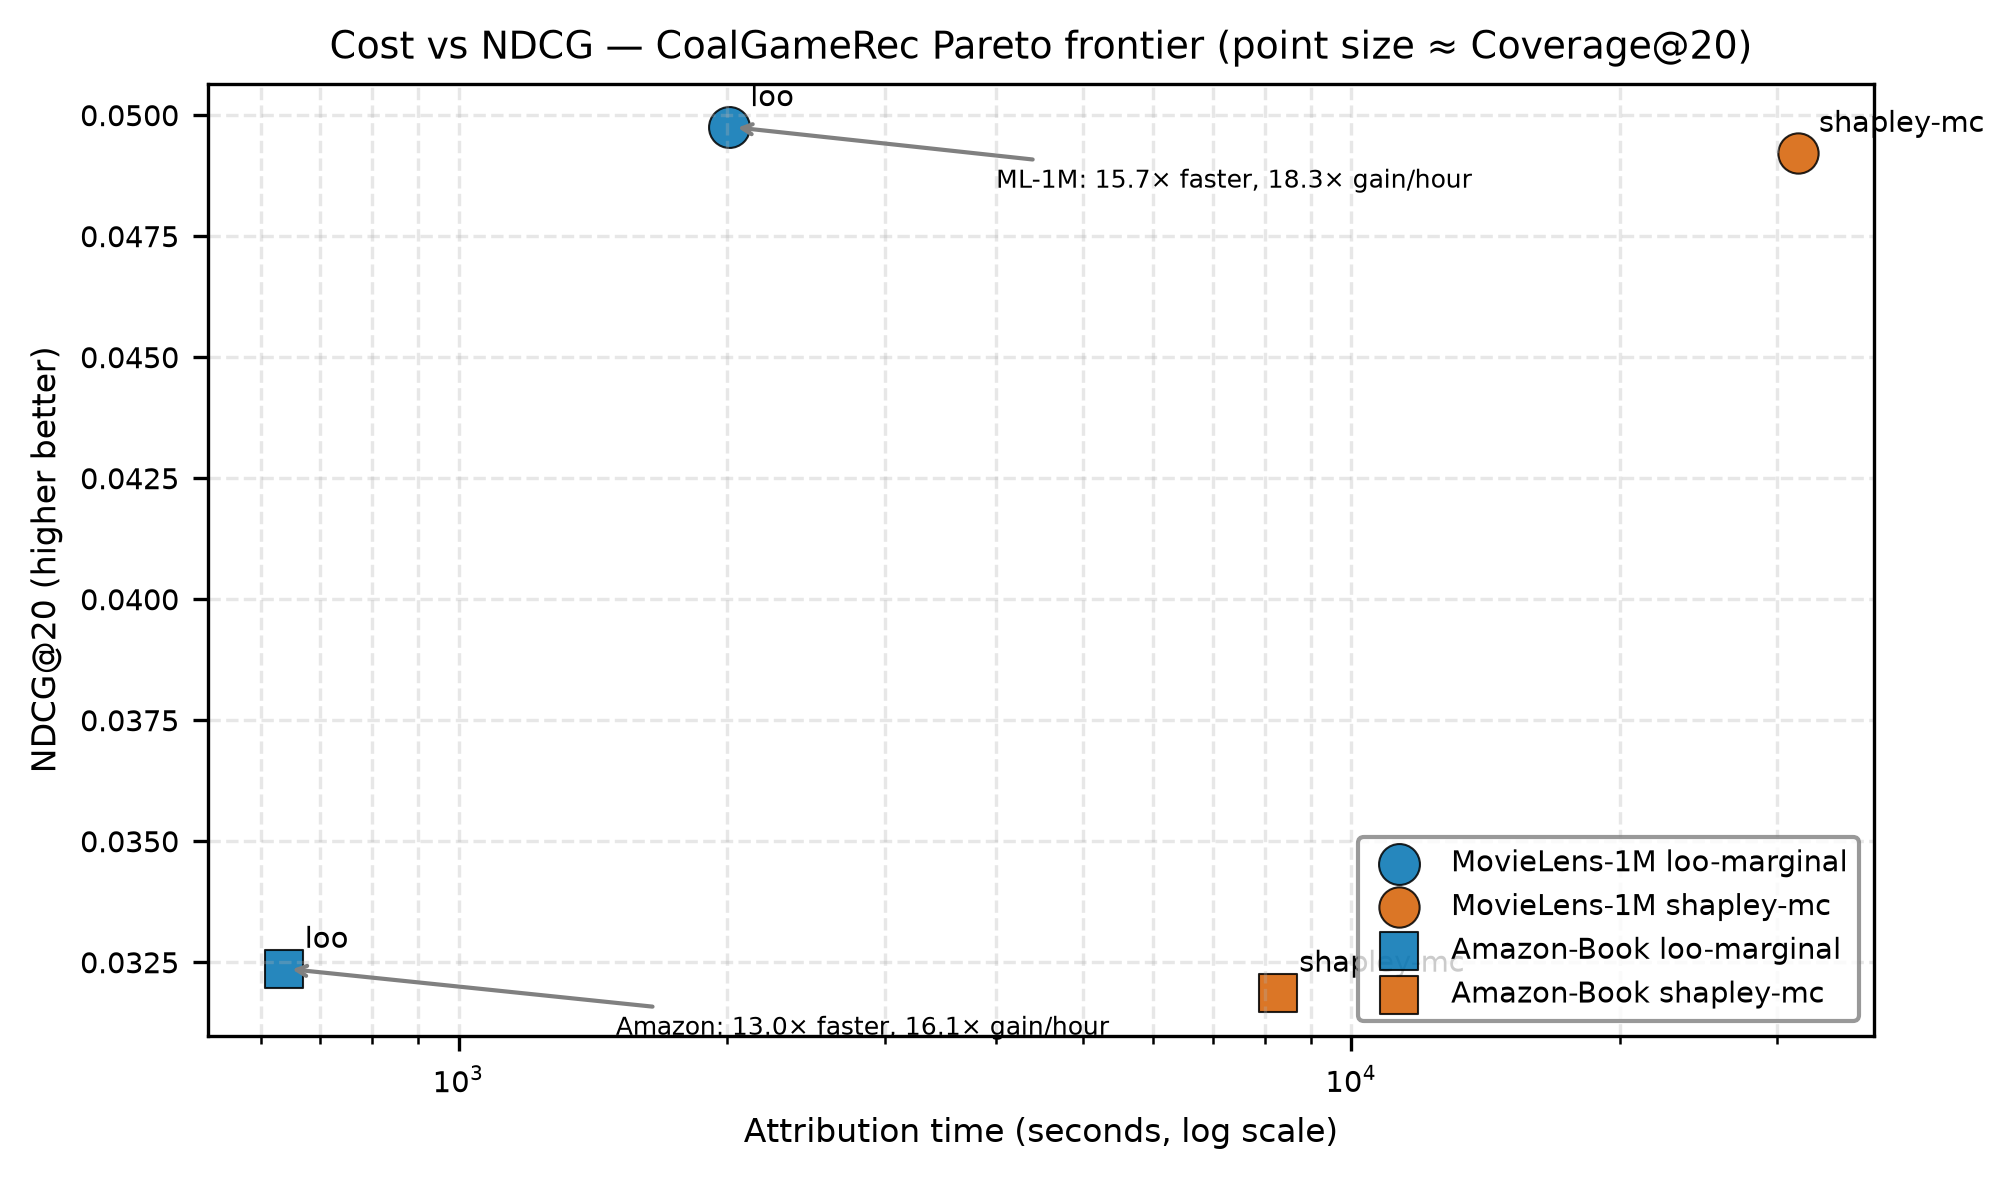
\includegraphics[width=0.85\textwidth]{assets/figures/cost_effectiveness.png}
\caption{Cost-effectiveness: NDCG@20 versus wall-clock attribution time (log scale). Point size encodes Coverage@20. LOO Pareto-dominates Shapley (higher NDCG, lower time); annotations show $13.0$--$15.7\times$ runtime and $16.1$--$18.3\times$ NDCG gain per hour (Table~\ref{tab:cost}). Attribution time excludes training and base-score caching.}
\label{fig:cost_schematic}
\end{figure*}

\subsection{Main LightGCN results}\label{subsec:main_results}

Table~\ref{tab:main_results} reports the main LightGCN results. The unreranked LightGCN (base scores $b_{ui}$, $\lambda_{\text{attr}}=0$) scores NDCG@20 $0.04482\pm0.00021$ on ML-1M and $0.02982\pm0.00074$ on Amazon ($\lambda=0$ rows of the released $\lambda$-sweep artifact, 5 seeds); every reranked method is compared at the same shared $\lambda_{\text{attr}}=0.10$. Validation-informed non-game controls (validation-similarity reweighting and a validation-tuned linear reranker) are not part of this primary frozen table; they were added in the confirmatory study C1 (\S\ref{subsec:c1}, Table~\ref{tab:c1_main}), which resolves the validation-access asymmetry empirically. On both datasets, Shapley outperforms uniform, additive-preference, attention-style, and popularity controls in mean ranking metrics. On MovieLens, Shapley achieves the highest HitRate@20, while LOO marginal achieves the highest NDCG@20, coverage, and ILD. On Amazon-Book, LOO marginal achieves the highest HitRate@20, NDCG@20, and coverage.

\begin{table*}[t]
\caption{Primary LightGCN test performance, mean $\pm$ SD over five seeds. Bold marks the best reranking result per dataset; paired tests are in Table~\ref{tab:paired}, and matched validation-informed controls are in Table~\ref{tab:c1_main}.}\label{tab:main_results}
\centering
\scriptsize
\resizebox{\textwidth}{!}{
\begin{tabular}{lllllll}
\toprule
Dataset & Backbone & Method & HitRate@20 & NDCG@20 & Coverage@20 & ILD@20 \\
\midrule
\multicolumn{7}{l}{\textit{MovieLens-1M --- unreranked reference ($\lambda_{\text{attr}}=0$)}}\\
MovieLens-1M & LightGCN & unreranked & 0.11415 $\pm$ 0.00100 & 0.04482 $\pm$ 0.00021 & 0.62967 $\pm$ 0.00312 & 0.73045 $\pm$ 0.00027 \\
\multicolumn{7}{l}{\textit{MovieLens-1M --- non-game reweighting (no validation access)}}\\
MovieLens-1M & LightGCN & uniform & 0.11737 $\pm$ 0.00102 & 0.04601 $\pm$ 0.00030 & 0.61452 $\pm$ 0.00196 & 0.72176 $\pm$ 0.00022 \\
MovieLens-1M & LightGCN & additive-pref & 0.11751 $\pm$ 0.00087 & 0.04610 $\pm$ 0.00020 & 0.61137 $\pm$ 0.00281 & 0.72011 $\pm$ 0.00026 \\
MovieLens-1M & LightGCN & attention & 0.11800 $\pm$ 0.00165 & 0.04648 $\pm$ 0.00046 & 0.60501 $\pm$ 0.00367 & 0.71703 $\pm$ 0.00021 \\
MovieLens-1M & LightGCN & heuristic-pop & 0.11754 $\pm$ 0.00110 & 0.04612 $\pm$ 0.00035 & 0.61040 $\pm$ 0.00231 & 0.72051 $\pm$ 0.00023 \\
\multicolumn{7}{l}{\textit{MovieLens-1M --- cooperative-game attribution (validation-guided)}}\\
MovieLens-1M & LightGCN & shapley-mc & 0.12555 $\pm$ 0.00084 & 0.04922 $\pm$ 0.00033 & 0.63372 $\pm$ 0.00396 & 0.72782 $\pm$ 0.00019 \\
MovieLens-1M & LightGCN & \textbf{CoalGameRec (LOO)} & \textbf{0.12519 $\pm$ 0.00230} & \textbf{0.04976 $\pm$ 0.00041} & \textbf{0.64123 $\pm$ 0.00296} & \textbf{0.73496 $\pm$ 0.00018} \\
\multicolumn{7}{l}{\textit{Amazon-Book --- unreranked reference ($\lambda_{\text{attr}}=0$)}}\\
Amazon-Book & LightGCN & unreranked & 0.06690 $\pm$ 0.00234 & 0.02982 $\pm$ 0.00074 & 0.23573 $\pm$ 0.00402 & 0.92082 $\pm$ 0.00143 \\
\multicolumn{7}{l}{\textit{Amazon-Book --- non-game reweighting (no validation access)}}\\
Amazon-Book & LightGCN & uniform & 0.06679 $\pm$ 0.00253 & 0.02978 $\pm$ 0.00078 & 0.23387 $\pm$ 0.00438 & \textbf{0.92104 $\pm$ 0.00142} \\
Amazon-Book & LightGCN & additive-pref & 0.06655 $\pm$ 0.00246 & 0.02968 $\pm$ 0.00075 & 0.23387 $\pm$ 0.00423 & 0.92091 $\pm$ 0.00144 \\
Amazon-Book & LightGCN & attention & 0.06604 $\pm$ 0.00249 & 0.02954 $\pm$ 0.00075 & 0.23454 $\pm$ 0.00388 & 0.92054 $\pm$ 0.00145 \\
Amazon-Book & LightGCN & heuristic-pop & 0.06687 $\pm$ 0.00284 & 0.02995 $\pm$ 0.00085 & 0.23379 $\pm$ 0.00433 & 0.92098 $\pm$ 0.00142 \\
\multicolumn{7}{l}{\textit{Amazon-Book --- cooperative-game attribution (validation-guided)}}\\
Amazon-Book & LightGCN & shapley-mc & 0.07019 $\pm$ 0.00289 & 0.03187 $\pm$ 0.00085 & 0.23424 $\pm$ 0.00394 & 0.92071 $\pm$ 0.00138 \\
Amazon-Book & LightGCN & \textbf{CoalGameRec (LOO)} & \textbf{0.07089 $\pm$ 0.00234} & \textbf{0.03237 $\pm$ 0.00077} & \textbf{0.23551 $\pm$ 0.00418} & 0.92038 $\pm$ 0.00145 \\
\bottomrule
\end{tabular}
}
\end{table*}

\subsection{Paired contrasts}\label{subsec:paired}

Table~\ref{tab:paired} reports the contrasts needed for the central claim; the complete pre-specified Holm families are provided with the released artifacts. Shapley beats uniform on both datasets, but it does not beat LOO. All standardized effects are negligible ($|d_z|<0.08$), so the practical claim rests on the equivalence interval and cost rather than statistical significance alone.

\begin{table*}[t]
\caption{Key paired contrasts ($B=2000$, Holm-adjusted within the pre-specified families). Negative Shapley--LOO differences favor LOO; complete contrast tables are released as artifacts.}\label{tab:paired}\label{tab:paired_loo}
\centering
\scriptsize
\resizebox{\textwidth}{!}{
\begin{tabular}{lllllll}
\toprule
Dataset & Contrast & Metric & Mean diff. & 95\% CI & $p$ & $d_z$ \\
\midrule
MovieLens-1M & Shapley vs uniform & NDCG@20 & 0.003216 & [0.002707, 0.003715] & $<0.0005$ & 0.0716 \\
MovieLens-1M & Shapley vs uniform & HitRate@20 & 0.008180 & [0.006517, 0.009875] & $<0.0005$ & 0.0550 \\
MovieLens-1M & Shapley vs LOO & NDCG@20 & -0.000532 & [-0.000963, -0.000119] & 0.008 & -0.0143 \\
MovieLens-1M & Shapley vs LOO & HitRate@20 & 0.000366 & [-0.000899, 0.001696] & 0.575 & 0.0032 \\
Amazon-Book & Shapley vs uniform & NDCG@20 & 0.002096 & [0.001703, 0.002474] & $<0.0005$ & 0.0568 \\
Amazon-Book & Shapley vs uniform & HitRate@20 & 0.003398 & [0.002427, 0.004395] & $<0.0005$ & 0.0348 \\
Amazon-Book & Shapley vs LOO & NDCG@20 & -0.000494 & [-0.000709, -0.000281] & $<0.0005$ & -0.0228 \\
Amazon-Book & Shapley vs LOO & HitRate@20 & -0.000701 & [-0.001375, -0.000054] & 0.036 & -0.0108 \\
\bottomrule
\end{tabular}
}
\end{table*}

The full LOO-as-treatment family also shows that LOO beats every non-game control on both metrics and datasets (all Holm $p<0.0005$). On HitRate@20, LOO and Shapley are indistinguishable on ML-1M ($p=0.575$), while LOO leads on Amazon-Book ($p=0.036$).

\subsection{Cost-effectiveness}\label{subsec:cost}

Table~\ref{tab:cost} compares offline attribution cost. The $10{,}160$\,s ML-1M Shapley run is retained in the reported mean and SD; no runtime observation was removed. Training and base-score caching add $1{,}402\pm27$\,s on ML-1M and $267\pm2$\,s on Amazon-Book. End-to-end serving latency and memory were not measured.

\begin{table*}[t]
\caption{Cost-effectiveness over five seeds. Attribution seconds report the five-seed total followed by per-seed mean $\pm$ SD in parentheses; training is excluded. Gain/hour uses the total attribution time.}\label{tab:cost}
\centering
\small
\resizebox{\textwidth}{!}{
\begin{tabular}{llllll}
\toprule
Dataset & Method & NDCG@20 & HitRate@20 & Attribution seconds & NDCG gain/hour \\
\midrule
MovieLens-1M & loo-marginal & 0.049755 & 0.125187 & 2010.5 ($402\pm5$) & 0.006712 \\
MovieLens-1M & shapley-mc & 0.049223 & 0.125553 & 31657.7 ($6332\pm2141$) & 0.000366 \\
Amazon-Book & loo-marginal & 0.032367 & 0.070891 & 637.2 ($127\pm1$) & 0.014630 \\
Amazon-Book & shapley-mc & 0.031873 & 0.070190 & 8283.2 ($1657\pm3$) & 0.000911 \\
\bottomrule
\end{tabular}
}
\end{table*}


\subsection{Equivalence of Shapley and LOO within a pre-specified margin}\label{subsec:equivalence}

Failure to reject a difference is not evidence of equality, so the ``match'' between Shapley and LOO is assessed with an explicit equivalence analysis rather than a non-significant p-value. The smallest effect size of practical interest (SESOI) was declared before computing the test: $\delta=0.001$ for NDCG@20 and $\delta=0.002$ for HitRate@20, approximately one quarter of the LOO-vs-uniform improvement under this protocol. Equivalence holds when the 90\% bootstrap percentile CI of the Shapley--LOO paired difference lies entirely inside $(-\delta,\delta)$ (Table~\ref{tab:equivalence}).

\begin{table}[t]
\caption{Equivalence analysis, Shapley-MC vs.\ LOO-marginal, paired user differences, 5 seeds, $B=2000$ (SESOI margins declared a priori; artifact: released equivalence tables of each v3 run). ``CI favors LOO'' = the entire 90\% CI is negative.}\label{tab:equivalence}
\centering
\resizebox{\textwidth}{!}{
\begin{tabular}{llllll}
\toprule
Dataset & Metric & Mean diff. & 90\% CI & Margin $\pm\delta$ & Equivalence / CI favors LOO \\
\midrule
ML-1M & NDCG@20 & $-0.000532$ & $[-0.000890,-0.000172]$ & $0.001$ & YES / YES \\
ML-1M & HitRate@20 & $+0.000366$ & $[-0.000698,+0.001496]$ & $0.002$ & YES / no \\
Amazon-Book & NDCG@20 & $-0.000494$ & $[-0.000680,-0.000309]$ & $0.001$ & YES / YES \\
Amazon-Book & HitRate@20 & $-0.000701$ & $[-0.001267,-0.000135]$ & $0.002$ & YES / YES \\
\bottomrule
\end{tabular}
}
\end{table}

Equivalence is established on all four contrasts. On NDCG@20 both intervals lie entirely below zero: within the practically negligible band, LOO is the preferred method on both datasets. On HitRate@20, ML-1M is equivalent without directional preference, while Amazon-Book favors LOO. We therefore replace ``LOO matches Shapley'' with the precise statement: \emph{Shapley provides no practically meaningful ranking improvement over LOO on NDCG@20 under this protocol, and the equivalence interval favors LOO.}

\subsection{Confirmatory matched-controls study (C1)}\label{subsec:c1}

The primary study compares validation-guided game attribution against non-game controls that have \emph{no} validation access, leaving open how much of the game-vs-heuristic gap is attributable to validation access itself. Study C1 closes this gap by adding two matched validation-informed non-game controls that consume the same validation item $i_u^+$ as the Shapley/LOO games but use no coalition structure:
\begin{itemize}
    \item \textbf{valid-sim}: history reweighting $w_j=\max(0,\cos(\mathbf{e}_j,\mathbf{e}_{i_u^+}))$ under the identical native intervention~(\ref{eq:rerank});
    \item \textbf{valid-linear}: candidate-side linear reranker $s'_{ui}=\mathrm{zscore}(b_{ui})+\lambda_{\text{attr}}\,\mathrm{zscore}(\cos(\mathbf{e}_i,\mathbf{e}_{i_u^+}))$, a strong matched non-game reranker with validation access.
\end{itemize}
Both share the a-priori $\lambda_{\text{attr}}=0.10$ and neither uses coalition values or attribution. C1 re-executes the frozen protocol (identical hyperparameters, seeds 42--46, archived splits; a scripted, notebook-driven pipeline; complete execution logs accompany each run) and, in its final version (C1b), also re-runs Shapley-MC under the identical matched environment, so all nine families are compared on the same re-executed models. Deviations from the v3 runs --- torch re-execution (both datasets on Apple MPS, torch 2.3.1), one shared propagation per batch (equivalent gradients), and the vectorized negative sampler --- are recorded in each run's manifest. As a fidelity check, C1 reproduces the primary study within seed noise: uniform NDCG@20 on ML-1M is $0.04601\pm0.00022$ (identical to v3), unreranked $0.04493\pm0.00018$ vs.\ v3 $0.04482\pm0.00021$, and LOO $0.04968\pm0.00038$ vs.\ v3 $0.04976\pm0.00041$.

Table~\ref{tab:c1_main} focuses on the matched comparison. Validation access improves over uniform, but LOO remains the strongest NDCG@20 method on both datasets.

\begin{table*}[t]
\caption{Confirmatory C1b ranking results, mean $\pm$ SD over five seeds. The table retains the uniform reference, matched validation-informed controls, and game-derived methods.}\label{tab:c1_main}
\centering
\small
\begin{tabular}{llcc}
\toprule
Dataset & Method & HitRate@20 & NDCG@20 \\
\midrule
ML-1M & uniform & 0.11741 $\pm$ 0.00091 & 0.04601 $\pm$ 0.00022 \\
ML-1M & valid-sim & 0.12190 $\pm$ 0.00086 & 0.04778 $\pm$ 0.00013 \\
ML-1M & valid-linear & 0.12316 $\pm$ 0.00087 & 0.04842 $\pm$ 0.00019 \\
ML-1M & Shapley & 0.12529 $\pm$ 0.00091 & 0.04909 $\pm$ 0.00030 \\
ML-1M & \textbf{LOO} & \textbf{0.12522 $\pm$ 0.00049} & \textbf{0.04968 $\pm$ 0.00038} \\
Amazon-Book & uniform & 0.06633 $\pm$ 0.00259 & 0.02945 $\pm$ 0.00080 \\
Amazon-Book & valid-sim & 0.06752 $\pm$ 0.00265 & 0.03035 $\pm$ 0.00073 \\
Amazon-Book & valid-linear & 0.07024 $\pm$ 0.00188 & 0.03154 $\pm$ 0.00058 \\
Amazon-Book & Shapley & 0.06984 $\pm$ 0.00225 & 0.03167 $\pm$ 0.00068 \\
Amazon-Book & \textbf{LOO} & \textbf{0.07111 $\pm$ 0.00265} & \textbf{0.03229 $\pm$ 0.00081} \\
\bottomrule
\end{tabular}
\end{table*}

Table~\ref{tab:c1_paired} reports the matched-control contrasts needed to assess validation access; the complete $F=12$ family is released with the artifacts. LOO beats both validation-informed controls on NDCG@20 on both datasets. The only non-significant retained contrast is Amazon HitRate@20 versus valid-linear ($p=0.086$).

Table~\ref{tab:c1_shap} presents the Shapley-focused NDCG@20 contrasts. Shapley beats valid-sim on both datasets and valid-linear on ML-1M, but is beaten by LOO on both datasets.

\begin{table*}[t]
\caption{C1b LOO contrasts against the validation-informed controls ($B=2000$, Holm-adjusted within the full $F=12$ family). Positive differences favor LOO.}\label{tab:c1_paired}
\centering
\scriptsize
\resizebox{\textwidth}{!}{
\begin{tabular}{lllllll}
\toprule
Dataset & Contrast & Metric & Mean diff. & 95\% CI & $p$ (Holm) & $d_z$ \\
\midrule

MovieLens-1M & LOO vs valid-sim & NDCG@20 & +0.001903 & [+0.001335, +0.002434] & $<0.0005$ (rej.) & 0.0394 \\
MovieLens-1M & LOO vs valid-linear & NDCG@20 & +0.001263 & [+0.000783, +0.001748] & $<0.0005$ (rej.) & 0.0303 \\
MovieLens-1M & LOO vs valid-sim & HitRate@20 & +0.003325 & [+0.001595, +0.004988] & $<0.0005$ (rej.) & 0.0221 \\
MovieLens-1M & LOO vs valid-linear & HitRate@20 & +0.002062 & [+0.000532, +0.003525] & 0.004 (rej.) & 0.0158 \\
Amazon-Book & LOO vs valid-sim & NDCG@20 & +0.001939 & [+0.001535, +0.002343] & $<0.0005$ (rej.) & 0.0481 \\
Amazon-Book & LOO vs valid-linear & NDCG@20 & +0.000754 & [+0.000370, +0.001131] & 0.001 (rej.) & 0.02 \\
Amazon-Book & LOO vs valid-sim & HitRate@20 & +0.003586 & [+0.002535, +0.004692] & $<0.0005$ (rej.) & 0.0331 \\
Amazon-Book & LOO vs valid-linear & HitRate@20 & +0.000863 & [$-$0.000135, +0.001861] & 0.086 (n.s.) & 0.0085 \\
\bottomrule
\end{tabular}
}
\end{table*}

\begin{table}[t]
\caption{Key C1b NDCG@20 contrasts with Shapley as treatment ($B=2000$, Holm-adjusted within the full $F=8$ family). Positive differences favor Shapley.}\label{tab:c1_shap}
\centering
\small
\begin{tabular}{llcc}
\toprule
Dataset & Comparator & Mean diff. & $p$ (Holm) \\
\midrule
ML-1M & valid-sim & +0.00131 & $<0.0005$ \\
ML-1M & valid-linear & +0.00067 & 0.002 \\
ML-1M & LOO & $-$0.00060 & 0.007 \\
Amazon-Book & valid-sim & +0.00131 & $<0.0005$ \\
Amazon-Book & valid-linear & +0.00013 & 0.441 \\
Amazon-Book & LOO & $-$0.00063 & $<0.0005$ \\
\bottomrule
\end{tabular}
\end{table}

\begin{table*}[t]
\caption{C1 masked-forward faithfulness evaluation with frozen LightGCN re-propagation after edge masking (single training seed per dataset). Deletion removes the highest-weighted history fraction; insertion retains only that fraction.}\label{tab:c1_faith}
\centering
\scriptsize
\resizebox{\textwidth}{!}{
\begin{tabular}{lllcc}
\toprule
Dataset & Weights & Fraction & Deletion NDCG@20 & Insertion NDCG@20 \\
\midrule
\multicolumn{5}{l}{\textit{MovieLens-1M --- unmasked reference: NDCG@20 $=0.04759$}}\\
MovieLens-1M & LOO & 0.1 & 0.04632 & 0.04894 \\
MovieLens-1M & LOO & 0.2 & 0.04603 & 0.04800 \\
MovieLens-1M & LOO & 0.3 & 0.04666 & 0.04742 \\
MovieLens-1M & Shapley & 0.1 & 0.04740 & 0.05176 \\
MovieLens-1M & Shapley & 0.2 & 0.04668 & 0.05029 \\
MovieLens-1M & Shapley & 0.3 & 0.04567 & 0.04875 \\
MovieLens-1M & uniform & 0.1 & 0.04772 & 0.04681 \\
MovieLens-1M & uniform & 0.2 & 0.04807 & 0.04829 \\
MovieLens-1M & uniform & 0.3 & 0.04695 & 0.04780 \\
MovieLens-1M & random & 0.1 & 0.04738 & 0.04876 \\
MovieLens-1M & random & 0.2 & 0.04760 & 0.04908 \\
MovieLens-1M & random & 0.3 & 0.04800 & 0.04708 \\
\multicolumn{5}{l}{\textit{Amazon-Book --- unmasked reference: NDCG@20 $=0.01723$}}\\
Amazon-Book & LOO & 0.1 & 0.01648 & 0.02162 \\
Amazon-Book & LOO & 0.2 & 0.01673 & 0.02015 \\
Amazon-Book & LOO & 0.3 & 0.01723 & 0.01951 \\
Amazon-Book & Shapley & 0.1 & 0.01540 & 0.02163 \\
Amazon-Book & Shapley & 0.2 & 0.01583 & 0.02024 \\
Amazon-Book & Shapley & 0.3 & 0.01623 & 0.02102 \\
Amazon-Book & uniform & 0.1 & 0.01674 & 0.01669 \\
Amazon-Book & uniform & 0.2 & 0.01659 & 0.01748 \\
Amazon-Book & uniform & 0.3 & 0.01615 & 0.01857 \\
Amazon-Book & random & 0.1 & 0.01748 & 0.01750 \\
Amazon-Book & random & 0.2 & 0.01731 & 0.01648 \\
Amazon-Book & random & 0.3 & 0.01779 & 0.01660 \\
\bottomrule
\end{tabular}
}
\end{table*}

\section{Sensitivity and diagnostic studies}\label{sec:ablation}
Table~\ref{tab:ablation_lambda} reports the reranking-strength sensitivity across the full five-seed protocol on both datasets, restricted to the families contained in the released $\lambda$-sweep artifact. The gain is not due to arbitrary reweighting: at $\lambda_{\text{attr}}=0$ all methods coincide with the base ranking (NDCG@20 $0.04482\pm0.00021$ on ML-1M; $0.02982\pm0.00074$ on Amazon). On ML-1M all families improve monotonically with $\lambda$, and Shapley rises fastest: at $\lambda=0.20$ it reaches $0.05278\pm0.00043$, $+7.2\%$ relative to its own value at the protocol setting $\lambda=0.10$ ($0.04922$) and $+6.1\%$ above LOO at $\lambda=0.10$ ($0.04976$, Table~\ref{tab:main_results}). We stress that $\lambda_{\text{attr}}=0.10$ was fixed a priori and shared across families; the sweep is a sensitivity analysis, not a selection rule, and per-family tuning is excluded by the protocol. On Amazon-Book the pattern is sharper: heuristic weights are flat across $\lambda$ (uniform stays within $0.02973$--$0.02982$; additive-pref weakly \emph{decreases}), while Shapley rises monotonically to $0.03591\pm0.00101$ at $\lambda=0.40$. This indicates that the Amazon gain is carried by the validation-guided game signal rather than by generic reweighting strength.

\begin{table}[t]
\caption{Reranking-strength sensitivity, NDCG@20, mean $\pm$ SD over five seeds on both datasets (families and values taken from the released $\lambda$-sensitivity artifacts; 5-seed values at the protocol $\lambda=0.10$ match Table~\ref{tab:main_results}). Bold column: protocol value $\lambda_{\text{attr}}=0.10$, fixed a priori and shared. The LOO family is not part of the released $\lambda$-sweep artifact and is reported only at the protocol value.}\label{tab:ablation_lambda}
\centering
\scriptsize
\resizebox{\textwidth}{!}{
\begin{tabular}{llccccc}
\toprule
Dataset & Family & $\lambda{=}0.00$ & $0.05$ & \textbf{$0.10$} & $0.20$ & $0.40$ \\
\midrule
ML-1M & uniform & 0.04482 $\pm$ 0.00021 & 0.04539 $\pm$ 0.00009 & \textbf{0.04601 $\pm$ 0.00030} & 0.04671 $\pm$ 0.00021 & 0.04793 $\pm$ 0.00033 \\
ML-1M & additive-pref & 0.04482 $\pm$ 0.00021 & 0.04545 $\pm$ 0.00015 & \textbf{0.04610 $\pm$ 0.00020} & 0.04714 $\pm$ 0.00025 & 0.04849 $\pm$ 0.00049 \\
ML-1M & shapley-mc & 0.04482 $\pm$ 0.00021 & 0.04698 $\pm$ 0.00019 & \textbf{0.04922 $\pm$ 0.00033} & 0.05278 $\pm$ 0.00043 & 0.05936 $\pm$ 0.00043 \\
Amazon-Book & uniform & 0.02982 $\pm$ 0.00074 & 0.02979 $\pm$ 0.00072 & \textbf{0.02978 $\pm$ 0.00078} & 0.02973 $\pm$ 0.00076 & 0.02975 $\pm$ 0.00087 \\
Amazon-Book & additive-pref & 0.02982 $\pm$ 0.00074 & 0.02973 $\pm$ 0.00073 & \textbf{0.02968 $\pm$ 0.00075} & 0.02957 $\pm$ 0.00077 & 0.02957 $\pm$ 0.00081 \\
Amazon-Book & shapley-mc & 0.02982 $\pm$ 0.00074 & 0.03097 $\pm$ 0.00089 & \textbf{0.03187 $\pm$ 0.00085} & 0.03376 $\pm$ 0.00083 & 0.03591 $\pm$ 0.00101 \\
\bottomrule
\end{tabular}
}
\end{table}

The bounded $k=24$ design keeps MC attribution feasible; the separate convergence study below evaluates $M\in\{16,32,64,128,256\}$. The retained $10{,}160$\,s ML-1M runtime observation motivates reporting both mean and SD rather than removing a system-level outlier post hoc.


\subsection{Design-factor ablations}\label{subsec:design_ablations}

Table~\ref{tab:design_ablations} reports descriptive single-seed point estimates from C1; no uncertainty or significance claim is attached to them. Performance is stable across $k\ge16$ in these runs, and the three player-selection variants have similar point estimates. Smooth pairwise utility exceeds hard top-$K$ utility for both families. The external kernel also exceeds the native intervention, especially on Amazon-Book, showing that model alignment is a semantic design choice rather than a guarantee of higher accuracy. These factors require a full multi-seed study before generalization.

\begin{table*}[t]
\caption{Design-factor ablations in the C1 environment (single training seed 42 per dataset; released design-ablation artifacts). NDCG@20. Intervention rows compare the native (protocol) intervention against the external train-only kernel.}\label{tab:design_ablations}
\centering
\scriptsize
\begin{tabular}{llllcc}
\toprule
Ablation & Variant & Family & & ML-1M & Amazon-Book \\
\midrule
Player budget $k$ & $k=8$  & LOO     & & 0.04942 & 0.03187 \\
                    & $k=8$  & Shapley & & 0.04867 & 0.03133 \\
                    & $k=16$ & LOO     & & 0.04976 & 0.03207 \\
                    & $k=16$ & Shapley & & 0.04909 & 0.03142 \\
                    & $k=24$ & LOO     & & 0.04912 & 0.03209 \\
                    & $k=24$ & Shapley & & 0.04892 & 0.03147 \\
                    & $k=32$ & LOO     & & 0.04948 & 0.03211 \\
                    & $k=32$ & Shapley & & 0.04900 & 0.03147 \\
\midrule
Player selection & stratified & Shapley & & 0.04892 & 0.03147 \\
                 & similarity & Shapley & & 0.04840 & 0.03149 \\
                 & random     & Shapley & & 0.04902 & 0.03146 \\
\midrule
Coalition utility & pairwise log-sigmoid & LOO     & & 0.04912 & 0.03209 \\
                  & pairwise log-sigmoid & Shapley & & 0.04892 & 0.03147 \\
                  & hard top-$K$ NDCG    & LOO     & & 0.04522 & 0.03063 \\
                  & hard top-$K$ NDCG    & Shapley & & 0.04610 & 0.03143 \\
\midrule
Intervention & native (protocol) & LOO     & & 0.04912 & 0.03209 \\
             & external kernel   & LOO     & & 0.05235 & 0.05439 \\
             & native (protocol) & Shapley & & 0.04892 & 0.03147 \\
             & external kernel   & Shapley & & 0.05037 & 0.05517 \\
\bottomrule
\end{tabular}
\end{table*}


\subsection{Synthetic redundancy and complementarity game}\label{subsec:redundancy_demo}

The redundancy mechanism is demonstrated directly on a synthetic coverage game with known ground-truth structure (Table~\ref{tab:redundancy_demo}): eight players covering four needs, with two redundant pairs ($a_1,a_2$ both cover need $A$; $b_1,b_2$ cover $B$), one complementary pair (need $C$ is covered only if \emph{both} $c_1$ and $c_2$ are present), one null player $z$, and one singleton $s$; the coalition value $v(S)$ is the fraction of needs covered. Exact Shapley ($2^8$ coalitions) and the grand-coalition LOO marginal are computed on the identical game. The outcome shows the expected mechanism: LOO assigns \emph{zero} to all four redundant players --- each is individually removable without loss because its partner still covers the need --- while Shapley splits their joint credit evenly ($0.125$ each; $0.50$ for the two pairs together). Symmetrically, LOO \emph{double-counts} the complementary pair (removing either member kills need $C$, so each receives its full value, $0.25+0.25=0.50$ where Shapley assigns $0.25$). The null player receives zero under both concepts. Consequently the LOO shares sum to $0.75$ against $v(N)=1.00$ --- a $-25\%$ efficiency gap --- while Shapley sums exactly to $1.00$ (residual $1.2\times10^{-15}$). This controlled instance shows that an LOO efficiency gap can arise from redundancy and complementarity rather than from a particular dataset.

\begin{table}[t]
\caption{Synthetic redundancy/complementarity coverage game (exact Shapley over $2^8$ coalitions vs.\ grand-coalition LOO; released synthetic demo artifacts). Redundant players are individually removable without loss; the complementary need requires both members.}\label{tab:redundancy_demo}
\centering
\small
\begin{tabular}{llcc}
\toprule
Item & Role & Shapley & LOO \\
\midrule
$a_1$, $a_2$ & redundant pair ($A$)   & $0.125$ each & $0.000$ each \\
$b_1$, $b_2$ & redundant pair ($B$)   & $0.125$ each & $0.000$ each \\
$c_1$, $c_2$ & complementary ($C$)    & $0.125$ each & $0.250$ each \\
$z$          & null player            & $0.000$      & $0.000$ \\
$s$          & singleton ($D$)        & $0.250$      & $0.250$ \\
\midrule
\multicolumn{2}{l}{Sum of shares vs.\ $v(N)=1.000$} & $1.000$ (residual $\sim10^{-15}$) & $0.750$ ($-25\%$ gap) \\
\bottomrule
\end{tabular}
\end{table}

\subsection{Shapley estimator convergence}\label{subsec:estimator_convergence}

Because the negative Shapley-vs-LOO result could in principle reflect an under-resolved Shapley estimator, Table~\ref{tab:estimator_convergence} reports an $M$-budget convergence study on ML-1M (user subsample of 1,000, two estimator RNG seeds per $M$, reference = mean of the two $M=256$ runs). The efficiency residual $|\sum_g\hat\phi_g-(v(P_u)-v(\emptyset))|$ is at machine precision ($\le4.3\times10^{-10}$) for every $M$, and the per-user attribution rank correlation with the $M=256$ reference rises monotonically from $0.81$ ($M=16$) to $0.96$ ($M=256$), passing $0.91$ at the protocol value $M=64$. The $M=64$ choice therefore captures the bulk of the estimator's ordering signal at a fraction of the $M=256$ cost, and the Shapley-vs-LOO ranking conclusion is stable across the two estimator seeds.

\begin{table}[t]
\caption{Shapley estimator convergence on ML-1M (1,000-user subsample, two estimator seeds; released convergence artifacts). Efficiency residual $=|\sum_g\hat\phi_g-(v(P_u)-v(\emptyset))|$; Spearman $\rho$ is the per-user attribution rank correlation with the $M=256$ reference.}\label{tab:estimator_convergence}
\centering
\small
\begin{tabular}{lccc}
\toprule
$M$ & Attribution time (s) & Efficiency residual & Spearman $\rho$ vs.\ $M=256$ \\
\midrule
16  & 296 / 280    & $3.6\times10^{-11}$ / $2.1\times10^{-11}$ & 0.807 / 0.818 \\
32  & 484 / 503    & $1.3\times10^{-10}$ / $1.0\times10^{-10}$ & 0.875 / 0.877 \\
64  & 900 / 898    & $3.0\times10^{-10}$ / $3.1\times10^{-10}$ & 0.913 / 0.914 \\
128 & 2337 / 1893  & $3.6\times10^{-10}$ / $3.9\times10^{-10}$ & 0.940 / 0.944 \\
256 & 17150 / 6716 & $4.3\times10^{-10}$ / $4.1\times10^{-10}$ & (reference) \\
\bottomrule
\end{tabular}
\end{table}

\subsection{Faithfulness scope}\label{sec:explainability}
Ranking improvement is not explanation faithfulness. The primary diagnostic is the C1 masked-forward comparison in Table~\ref{tab:c1_faith}, which removes edges, renormalizes degrees, and re-propagates the frozen model. It suggests that LOO and Shapley select influential history more effectively than uniform or random weights, but it uses one training seed per dataset and has no confidence intervals. Given known weaknesses of perturbation fidelity under graph distribution shift \cite{zheng2024robust,fang2023evaluating}, we do not claim full faithfulness without multi-seed curves, stability tests, model randomization, and user-centered evaluation.
\section{Discussion}\label{sec:discussion}
The results have three levels. First, validation-guided game signals improve ranking over uniform and similarity-style reweighting. Second, full coalition-context averaging is not necessary for NDCG@20 under the evaluated protocol: LOO is equivalent within the declared margin, directionally favored, and $13.0$--$15.7\times$ cheaper. Third, ranking utility does not establish explanation faithfulness. The single-seed masked-forward results are diagnostic rather than conclusive.

The synthetic game clarifies why Shapley may still matter. It distributes credit across redundant players and avoids the LOO overcounting of complementary players, whereas the real-data ranking task does not reward this distinction enough to offset cost. Shapley should therefore be justified by interaction sensitivity, stability, or user-facing explanation quality rather than by axioms alone.

Although paired tests are significant, all standardized effects are below $0.08$, well below conventional ``small'' standardized-effect thresholds \cite{cohen1988power}. The absolute NDCG@20 gains are also modest. We therefore interpret the main contribution as a computational boundary result, not evidence of large deployment impact.

\subsection{Limitations and required extensions}\label{sec:negative_result}\label{sec:how_to_read}\label{sec:final_framing}\label{sec:future_work}\label{sec:threats}\label{sec:limitations}
The evidence is limited to LightGCN, MovieLens-1M, and a custom temporal Amazon-Book split; no external explainable-recommendation method is evaluated. Generalization requires at least a second backbone, another domain, and counterfactual or influence-function baselines. The design-factor and masked-forward studies use one training seed per dataset and therefore need multi-seed intervals before supporting robust claims.

Inference is conditional on five trained models. The current artifacts do not include seed-population inference, Friedman/Nemenyi omnibus comparisons, complementary Wilcoxon tests, or a formal equivalence-test power analysis. These analyses, together with the proportion of users whose test item crosses the top-20 boundary, would improve practical interpretation. The protocol comparison is also parameter-dependent: Shapley exceeds LOO at larger reranking weights on ML-1M, $k=24$ bounds the player set, and $M=64$ is validated only on a 1,000-user convergence subset. Finally, cost results cover offline attribution only; serving latency, memory, and the retained runtime outlier require dedicated profiling.


\section{Conclusion}\label{sec:conclusion}

This paper argues that cooperative-game attribution should be treated as a precise design language rather than a guaranteed performance enhancer. The LightGCN case study shows that a carefully specified bounded Shapley intervention improves ranking over uniform and similarity-based controls on MovieLens-1M and Amazon-Book. However, leave-one-out marginal attribution captures most or all of the ranking benefit at a fraction of the computational cost. This boundary condition is central: the axiomatic appeal of Shapley does not by itself justify its use unless coalition-context averaging adds measurable ranking, explanation, stability, or interaction-sensitive benefits beyond simpler marginal baselines.

Within the evaluated protocol, LOO is the computationally preferred validation-guided reranker; Shapley is justified only when follow-up masked-forward faithfulness or interaction-sensitivity results demonstrate benefits that offset its $13.0$--$15.7\times$ attribution-time cost.



\section*{Declarations}

\subsection*{Competing interests}
M.\ Louhichi is author of prior works on Shapley-based explanations \cite{louhichi2023shapleyclustering,louhichi2025gametheoryxai} and of the DyHuCoG hypergraph recommender \cite{louhichi2026dyhucog}, which is discussed only as a literature taxonomy example and is not used as the empirical backbone. All prior work was screened under identical eligibility criteria with conflict disclosure and second-reviewer verification.

\subsection*{Ethics approval and consent to participate}
The case study uses secondary public/pseudonymous datasets (MovieLens-1M \cite{harper2015movielens} and Amazon Reviews 2018 Books 5-core \cite{ni2019justifying}). Only ratings, item/user identifiers (remapped to integers), and timestamps were used; raw review text, demographics, and free-text content were not processed. No new user study was conducted. Institutional determination was obtained (exempt, 2026-07-15, ENSIAS IRB 2026-07-CoalGameRec); identifiers are not redistributed and split files use remapped integer IDs where archived.

\subsection*{Data availability}
MovieLens-1M and Amazon Reviews 2018 Books are public. Raw data are not redistributed. Preprocessing and split-generation code, resolved configs, dataset statistics, item-vector fingerprints, and SHA256 hashes are in the repository; large splits and per-user metrics are archived externally upon acceptance (Zenodo DOI to be minted from the tagged release; SHA256 checksums and download instructions are in Supplementary File S2; reviewers may access the anonymized repository snapshot at the submission commit).

\subsection*{Author contributions}
M.\ Louhichi: conceptualization, methodology, software, investigation, writing -- original draft. R.\ Nesmaoui: supervision, methodology, writing -- review \& editing. M.\ Lazaar: supervision, writing -- review \& editing. All CRediT roles confirmed.

\bibliography{references}

\end{document}
